% ---------------------------------------------------------------------------- %
\subsection{Versuchsanordnung}
\label{subsec:versuchsanordnung}
% ---------------------------------------------------------------------------- %

Die       Versuchsanordnung      ist       schematisch      in       Abbildung
\ref{fig:versuchsanordnung} dargestellt.

\begin{figure}[h!]
    \centering
    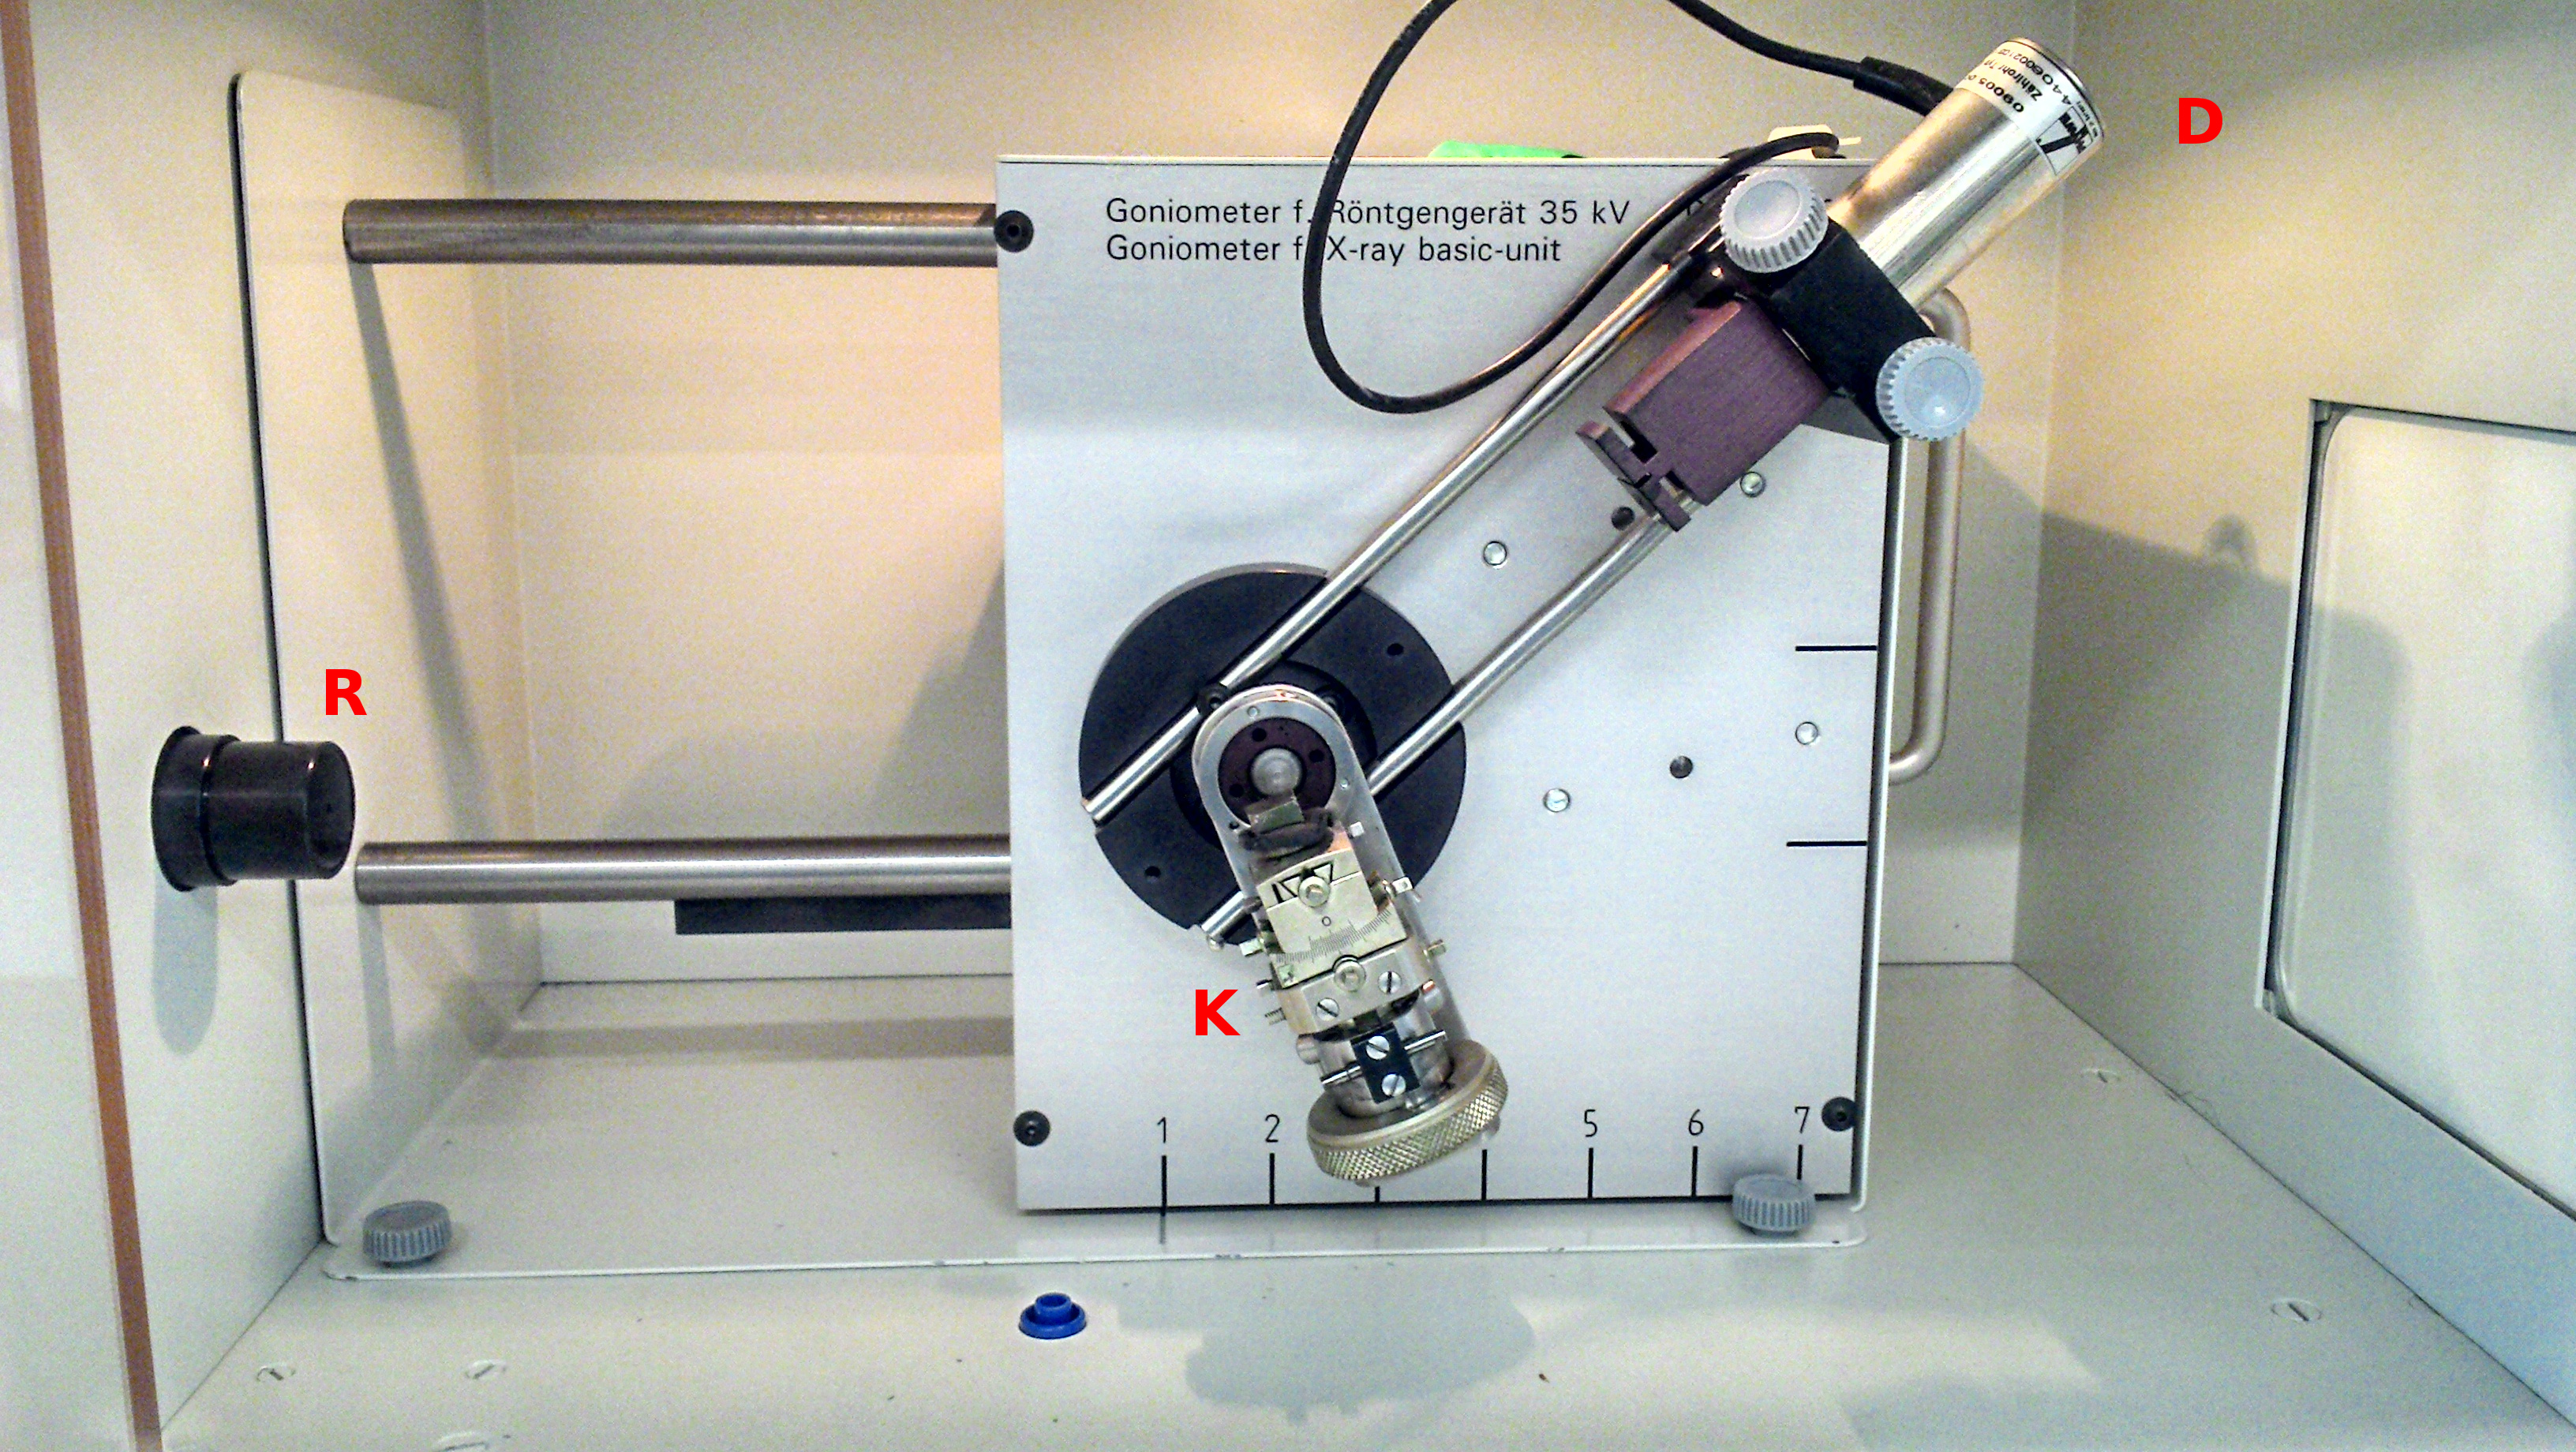
\includegraphics[width=.8\textwidth]{images/versuchsanordnung.jpg}
    \caption{%
        Versuchsanordnung.    \textbf{R}: Austritt   der    R\"ontgenstrahlung
        aus  dem   Bleikollimator,  \textbf{K}: Drehhalterung   mit  Kristall,
        \textbf{D}: Detektor
    }
    \label{fig:versuchsanordnung}
\end{figure}

Der   Detektor   rotiert   dabei   stets  mit   dem   doppelten   Winkel   der
Kristallhalterung  um den  Mittelpunkt. Daher ist  in den  Plots im  folgenden
Kapitel jeweils der Z\"ahlrohrwinkel gleich dem doppelten Glanzwinkel.

In Abbildung \ref{fig:roehre} ist eine der benutzten auswechselbaren Einheiten
mit einer R\"ontgenr\"ohre zu sehen.

\vspace{-0.5em}

\begin{figure}[h!]
    \centering
    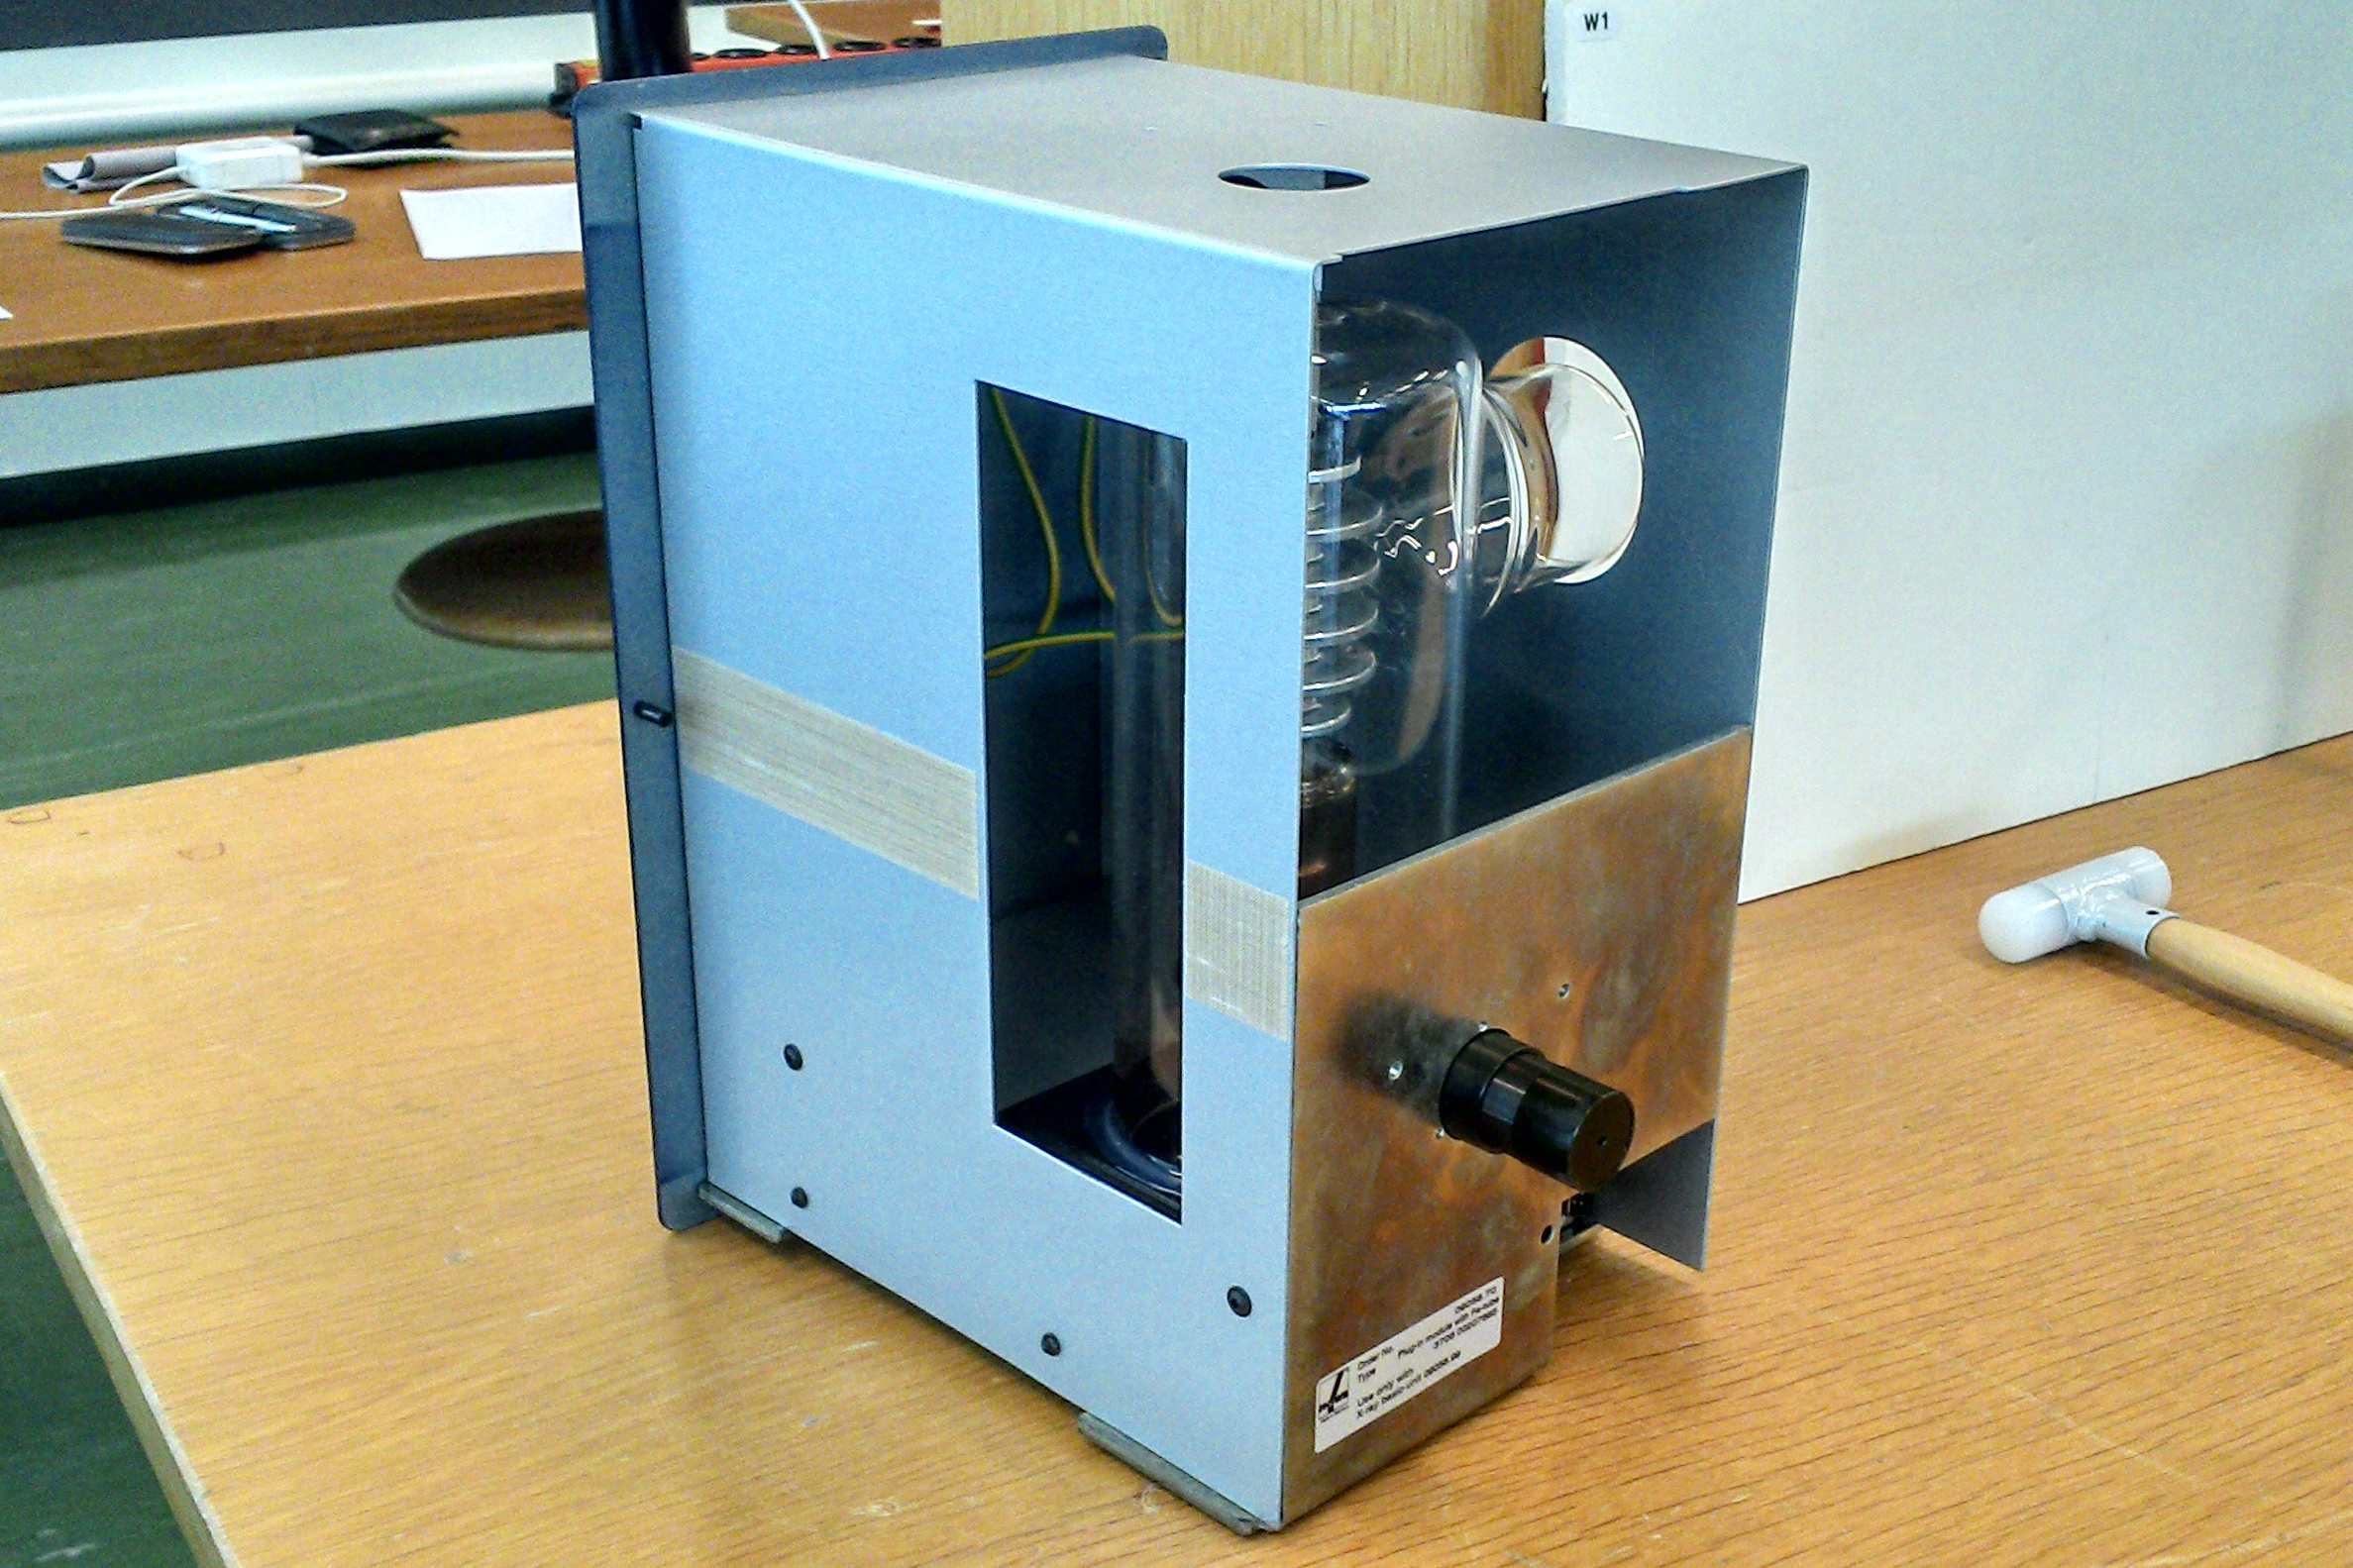
\includegraphics[width=.55\textwidth]{images/roehre.jpg}
    \caption{%
        Eine der benutzten R\"ontgenr\"ohren-Einheiten
    }
    \label{fig:roehre}
\end{figure}


\clearpage
% ---------------------------------------------------------------------------- %
\subsection{Ger\"ateliste}
\label{subsec:deviceList}
% ---------------------------------------------------------------------------- %

Die verwendeten Ger\"ate sind in Tabelle \ref{tab:deviceList} aufgef\"uhrt.

\captionof{table}{Hilfsmittel und Ger\"ateliste}
\label{tab:deviceList}
\begin{tabular}{ll}
    \toprule
    Ger\"at & Typ \\
    \midrule
    R\"ontgenger\"at & Phywe, \SI{35}{\kilo\volt} \\
    R\"ontgenr\"ohre & Phywe, Kupferanode \\
    R\"ontgenr\"ohre & Phywe, Eisenanode \\
    R\"ontgenr\"ohre & Phywe, Molybd\"ananode \\
    Auswerteprogramm Versuchsapparatur              & Phywe Measure \\
    Auswerteprogramm Bericht              & QtiPlot \\
    \bottomrule
\end{tabular}


% ---------------------------------------------------------------------------- %
\subsection{Messvorgang/Messmethoden}
\label{subsec:measurementMethods}
% ---------------------------------------------------------------------------- %

Es    wurde    die    gew\"unschte     R\"ohre    und    der    Bleikollimator
eingesetzt. Anschliessend  wurde   auf  der   rotierenden  Halterung   der  zu
analysierende  Kristall befestigt. Die  Apparatur  wurde  justiert und  danach
wurde die Messung via PC-Software automatisiert durchgef\"uhrt.

% ---------------------------------------------------------------------------- %
\subsection{Proben/Versuchsobjekte}
\label{subsec:samples}
% ---------------------------------------------------------------------------- %

Es wurden folgende Kristalle untersucht:
\begin{itemize}
    \item
        LiF
    \item
        Bergkristall (SiO)
    \item
        Kalkspat (Kalzit, CaCO3)
    \item
        Pyrit (Katzengold, FeS2)
    \item
        synthetischer Quartz (SiO2)
\end{itemize}

% ---------------------------------------------------------------------------- %
%\subsection{Messungen}
%\label{subsec:measurements}
% ---------------------------------------------------------------------------- %
